\chapter{PHÂN TÍCH VÀ THIẾT KẾ CƠ SỞ DỮ LIỆU PHÂN TÁN}

\section{Mô hình phân tán theo chi nhánh và số liệu giả định}

\subsection{Lý do phân tán và mô hình mạng trạm}
Giải bóng đá chuyên nghiệp có các trận đấu diễn ra phân bố tại nhiều tỉnh thành trên cả nước. Việc lưu trữ toàn bộ dữ liệu tập trung tại một máy chủ duy nhất sẽ làm tăng tải đường truyền mạng diện rộng khi các ban tổ chức sân đồng thời gửi danh sách đăng ký thi đấu và cập nhật diễn biến sự kiện trực tiếp theo từng phút. Hơn nữa, việc phân tán dữ liệu theo khu vực địa lý giúp tăng cường tính sẵn sàng, giảm độ trễ truy vấn tại từng cụm sân và cô lập bảo mật đối với dữ liệu tài chính bán vé.

Hệ thống được thiết kế phân tán trên ba trạm kết nối qua mạng riêng ảo:
\begin{itemize}
    \item \textbf{Trạm Trung tâm (Trụ sở Liên đoàn và Ban Tổ chức giải -- Trạm 0)}: Quản lý tổng thể giải đấu, nắm giữ bản gốc của toàn bộ các bảng danh mục, lưu trữ độc quyền mảnh tài chính thương mại bán vé (\texttt{TRAN\_DAU\_DOANH\_THU}) để kiểm toán và hạch toán doanh thu các sân thi đấu, tính toán thù lao trọng tài và tổng hợp bảng xếp hạng chung cuộc toàn mùa giải.
    \item \textbf{Chi nhánh Miền Bắc (Ban điều hành khu vực phía Bắc -- Trạm 1)}: Quản lý trực tiếp các sân vận động có thuộc tính $\text{KhuVuc} = \text{'MienBac'}$ (gồm Sân Hàng Đẫy, Sân Quốc gia Mỹ Đình, Sân Lạch Tray và Sân Thiên Trường) cùng toàn bộ dữ liệu chuyên môn của 25 trận đấu diễn ra tại miền Bắc.
    \item \textbf{Chi nhánh Miền Nam (Ban điều hành khu vực phía Nam -- Trạm 2)}: Quản lý trực tiếp các sân vận động có thuộc tính $\text{KhuVuc} = \text{'MienNam'}$ (gồm Sân Pleiku) cùng toàn bộ dữ liệu chuyên môn của 5 trận đấu diễn ra tại miền Nam.
\end{itemize}

\subsection{Số liệu giả định tần suất truy vấn}
Để phân tích chiến lược phân mảnh và nhân bản hợp lý, xét chu kỳ một vòng đấu gồm 3 trận diễn ra vào cuối tuần với số liệu giả định về tần suất thực thi các ứng dụng tại ba trạm được trình bày trong Bảng~\ref{tab:tan_suat_ung_dung}:

\begin{table}[H]
\centering
\small
\begin{tabular}{|l|p{6.5cm}|c|c|c|}
\hline
\textbf{Ứng dụng} & \textbf{Mô tả thao tác nghiệp vụ} & \textbf{Chi nhánh Bắc} & \textbf{Chi nhánh Nam} & \textbf{Trung tâm} \\ \hline
Ứng dụng 1 & Tra cứu danh mục đội bóng, cầu thủ, hợp đồng, màu áo & 800 lần & 300 lần & 100 lần \\ \hline
Ứng dụng 2 & Đăng ký danh sách thi đấu 18 cầu thủ trước trận & 20 lần & 10 lần & 0 lần \\ \hline
Ứng dụng 3 & Ghi nhận tỉ số, sự kiện bàn thắng, thẻ phạt trực tiếp & 150 lần & 50 lần & 10 lần \\ \hline
Ứng dụng 4 & Tổng hợp bảng xếp hạng và thống kê vua phá lưới & 20 lần & 10 lần & 80 lần \\ \hline
Ứng dụng 5 & Kiểm toán doanh thu bán vé sân và thù lao trọng tài & 0 lần & 0 lần & 60 lần \\ \hline
\end{tabular}
\caption{Bảng số liệu giả định tần suất ứng dụng tại các trạm trong một vòng đấu}
\label{tab:tan_suat_ung_dung}
\end{table}

Số liệu định lượng cho thấy: (1) Các bảng danh mục có tỷ lệ đọc trên ghi vượt mức $99\%$ trong suốt mùa giải; (2) Các thao tác đăng ký đội hình và cập nhật sự kiện trận đấu mang tính cục bộ tuyệt đối tại chi nhánh quản lý sân tổ chức trận đấu; (3) Nghiệp vụ kiểm toán giá vé và số lượng khán giả chỉ thực hiện tập trung tại Trạm Trung tâm.

\section{Thiết kế các phân mảnh dữ liệu và chứng minh tính đúng đắn}

Hệ thống áp dụng mô hình phân mảnh hỗn hợp kết hợp phân mảnh dọc, phân mảnh ngang nguyên thủy theo thuộc tính khu vực, chuỗi phân mảnh ngang dẫn xuất hai cấp và nhân bản bất đồng bộ Chủ -- Tớ.

\subsection{Phân mảnh dọc quan hệ TRAN\_DAU}
Quan hệ \texttt{TRAN\_DAU} gồm 15 thuộc tính được phân mảnh dọc thành hai quan hệ con dựa trên sự tách biệt giữa nghiệp vụ điều hành chuyên môn sân cỏ và nghiệp vụ kiểm toán tài chính thương mại:
\begin{itemize}
    \item \textbf{Mảnh chuyên môn điều hành trận đấu} ($\text{TRAN\_DAU\_CHUYEN\_MON} = \pi_{A_1}(\text{TRAN\_DAU})$):
    \begin{align*}
        A_1 = \{&\underline{\mathbf{MaTran}}, \text{MaVong}, \text{MaDoiNha}, \text{MaDoiKhach}, \text{MaSan}, \text{NgayGio}, \text{BanThangNha}, \\
        &\text{BanThangKhach}, \text{TheVangNha}, \text{TheVangKhach}, \text{TheDoNha}, \text{TheDoKhach}, \text{TrangThai}\}.
    \end{align*}
    \item \textbf{Mảnh tài chính doanh thu bán vé} ($\text{TRAN\_DAU\_DOANH\_THU} = \pi_{A_2}(\text{TRAN\_DAU})$):
    $$A_2 = \{\underline{\mathbf{MaTran}}, \text{GiaVe}, \text{SoKhach}\}.$$
\end{itemize}

\textbf{Chứng minh ba điều kiện đúng đắn của phân mảnh dọc:}
\begin{enumerate}
    \item \textit{Tính đầy đủ}: Hợp hai tập thuộc tính thỏa mãn $A_1 \cup A_2 = U_{\text{TRAN\_DAU}}$ (đầy đủ 15 thuộc tính).
    \item \textit{Tính tách biệt}: Giao của hai tập thuộc tính chỉ chứa duy nhất khóa chính của quan hệ gốc: $A_1 \cap A_2 = \{\text{MaTran}\}$; tập các thuộc tính không khóa hoàn toàn rời nhau.
    \item \textit{Tính tái thiết}: Vì $\text{MaTran}$ là khóa chính của cả hai mảnh dọc, phép kết nối tự nhiên trên $\text{MaTran}$ bảo toàn không mất mát thông tin:
    $$\text{TRAN\_DAU} = \text{TRAN\_DAU\_CHUYEN\_MON} \bowtie_{\text{MaTran}} \text{TRAN\_DAU\_DOANH\_THU}.$$
\end{enumerate}
Mảnh $\text{TRAN\_DAU\_DOANH\_THU}$ được định vị độc quyền tại Trạm Trung tâm; trong khi mảnh $\text{TRAN\_DAU\_CHUYEN\_MON}$ tiếp tục được phân mảnh ngang dẫn xuất về hai chi nhánh miền.

\subsection{Phân mảnh ngang nguyên thủy quan hệ SAN\_VAN\_DONG}
Quan hệ \texttt{SAN\_VAN\_DONG} được phân mảnh ngang nguyên thủy dựa trên thuộc tính phân vùng địa lý \texttt{KhuVuc} thay vì liệt kê cứng mã định danh sân, đảm bảo khi giải đấu mở rộng thêm sân vận động mới thì quy tắc phân mảnh vẫn tự động hiệu lực:
\begin{itemize}
    \item Vị từ $p_1$: $\text{KhuVuc} = \text{'MienBac'}$
    \item Vị từ $p_2$: $\text{KhuVuc} = \text{'MienNam'}$
\end{itemize}
Hai mảnh ngang nguyên thủy được xác định bởi phép chọn:
\begin{align*}
    \text{SAN\_VAN\_DONG}_1 &= \sigma_{\text{KhuVuc} = \text{'MienBac'}}(\text{SAN\_VAN\_DONG}) \quad (\text{đặt tại Chi nhánh Miền Bắc}), \\
    \text{SAN\_VAN\_DONG}_2 &= \sigma_{\text{KhuVuc} = \text{'MienNam'}}(\text{SAN\_VAN\_DONG}) \quad (\text{đặt tại Chi nhánh Miền Nam}).
\end{align*}

\textbf{Chứng minh ba điều kiện đúng đắn của phân mảnh ngang nguyên thủy:}
\begin{enumerate}
    \item \textit{Tính đầy đủ}: Do ràng buộc toàn vẹn miền giá trị \texttt{CHECK (KhuVuc IN ('MienBac', 'MienNam'))} trên bảng \texttt{SAN\_VAN\_DONG}, mọi bộ dữ liệu đều thỏa mãn $p_1 \lor p_2 = \text{TRUE}$.
    \item \textit{Tính tách biệt}: Hai vị từ $p_1$ và $p_2$ xung khắc từng đôi ($p_1 \land p_2 = \text{FALSE}$), suy ra $\text{SAN\_VAN\_DONG}_1 \cap \text{SAN\_VAN\_DONG}_2 = \emptyset$.
    \item \textit{Tính tái thiết}: Quan hệ gốc được khôi phục đầy đủ bằng phép hợp:
    $$\text{SAN\_VAN\_DONG} = \text{SAN\_VAN\_DONG}_1 \cup \text{SAN\_VAN\_DONG}_2.$$
\end{enumerate}

\subsection{Chuỗi phân mảnh ngang dẫn xuất hai cấp}

\paragraph{Cấp 1 -- Phân mảnh dẫn xuất quan hệ TRAN\_DAU\_CHUYEN\_MON:}
Do quan hệ $\text{TRAN\_DAU\_CHUYEN\_MON}$ không lưu thuộc tính $\text{KhuVuc}$ mà tham chiếu tới $\text{SAN\_VAN\_DONG}$ qua khóa ngoại $\text{MaSan}$, ta áp dụng phép bán kết nối để phân mảnh dẫn xuất $\text{TRAN\_DAU\_CHUYEN\_MON}$ theo $\text{SAN\_VAN\_DONG}_i$ ($i \in \{1, 2\}$):
$$\text{TRAN\_DAU\_CHUYEN\_MON}_1 = \text{TRAN\_DAU\_CHUYEN\_MON} \ltimes_{\text{MaSan}} \text{SAN\_VAN\_DONG}_1$$
$$\text{TRAN\_DAU\_CHUYEN\_MON}_2 = \text{TRAN\_DAU\_CHUYEN\_MON} \ltimes_{\text{MaSan}} \text{SAN\_VAN\_DONG}_2$$
Vì $\text{MaSan}$ là khóa ngoại không rỗng tham chiếu tới khóa chính của $\text{SAN\_VAN\_DONG}$ và $\{\text{SAN\_VAN\_DONG}_1, \text{SAN\_VAN\_DONG}_2\}$ là một phân hoạch đầy đủ, rời nhau, nên $\{\text{TRAN\_DAU\_CHUYEN\_MON}_1, \text{TRAN\_DAU\_CHUYEN\_MON}_2\}$ cũng thỏa mãn tuyệt đối tính đầy đủ ($25 + 5 = 30$ trận), tính tách biệt ($\text{TRAN\_DAU\_CHUYEN\_MON}_1 \cap \text{TRAN\_DAU\_CHUYEN\_MON}_2 = \emptyset$) và tính tái thiết bằng phép hợp.

\paragraph{Cấp 2 -- Phân mảnh dẫn xuất các quan hệ sự kiện và đăng ký:}
Các quan hệ phụ thuộc trực tiếp vào khóa ngoại $\text{MaTran}$ được phân mảnh ngang dẫn xuất cấp 2 thông qua phép bán kết nối với $\text{TRAN\_DAU\_CHUYEN\_MON}_i$ ($i \in \{1, 2\}$):
\begin{align*}
    \text{PHAN\_CONG\_TRONG\_TAI}_i &= \text{PHAN\_CONG\_TRONG\_TAI} \ltimes_{\text{MaTran}} \text{TRAN\_DAU\_CHUYEN\_MON}_i \\
    \text{DANG\_KY\_THI\_DAU}_i &= \text{DANG\_KY\_THI\_DAU} \ltimes_{\text{MaTran}} \text{TRAN\_DAU\_CHUYEN\_MON}_i \\
    \text{SU\_KIEN\_TRAN\_DAU}_i &= \text{SU\_KIEN\_TRAN\_DAU} \ltimes_{\text{MaTran}} \text{TRAN\_DAU\_CHUYEN\_MON}_i
\end{align*}
Cách thiết kế này bảo đảm toàn bộ chuỗi khóa ngoại từ $\text{SU\_KIEN\_TRAN\_DAU}_i \rightarrow \text{DANG\_KY\_THI\_DAU}_i \rightarrow \text{TRAN\_DAU\_CHUYEN\_MON}_i \rightarrow \text{SAN\_VAN\_DONG}_i$ đều nằm trọn vẹn trong cùng một trạm khu vực.

\textit{Cơ chế kiểm soát ràng buộc toàn vẹn trong môi trường phân tán}:
\begin{itemize}
    \item \textbf{Ràng buộc nội bộ trận đấu}: Các kiểm tra về biên chế đăng ký trong trận (11 đá chính, tối đa 7 dự bị), đối soát tỉ số và tổng số thẻ trong trận được thực thi cục bộ tức thì tại từng chi nhánh mà không cần truy vấn xuyên mạng.
    \item \textbf{Ràng buộc toàn cục liên trạm}: Các quy tắc liên quan đến việc cầu thủ/đội bóng di chuyển thi đấu giữa hai miền (như án treo giò phát sinh từ trận làm khách ở miền Nam nhưng trận kế tiếp đá tại miền Bắc) hoặc trọng tài bắt trận ở cả hai miền trong cùng một vòng đấu là các ràng buộc toàn cục (Global Constraints). Trong giải pháp phân tán của PostgreSQL, Trạm Trung tâm thiết lập khung nhìn toàn cục hợp nhất \texttt{vw\_global\_su\_kien\_tran\_dau} và \texttt{vw\_global\_dang\_ky\_thi\_dau} thông qua liên kết \texttt{postgres\_fdw} tới các chi nhánh. Khi tiếp nhận danh sách đăng ký thi đấu, trigger tại chi nhánh truy vấn Foreign View toàn cục tại Trạm Trung tâm để đối soát lịch sử thẻ phạt và án kỷ luật trên toàn quốc, bảo đảm việc kiểm soát treo giò luôn chính xác tuyệt đối mà không cần duy trì bảng trung gian thủ công.
    \item \textbf{Kiểm soát sức chứa khi phân mảnh dọc}: Thuộc tính \texttt{SoKhach} nằm ở mảnh doanh thu tại Trạm 0, do đó quy định kiểm soát số lượng khán giả không vượt quá sức chứa được thực thi tại Trạm Trung tâm khi kết nối mảnh \texttt{TRAN\_DAU\_DOANH\_THU} với bản sao nhân bản của \texttt{SAN\_VAN\_DONG}.
\end{itemize}

\subsection{Cơ chế nhân bản bất đồng bộ Chủ -- Tớ cho các bảng danh mục}
Sáu bảng danh mục gồm \texttt{DOI\_BONG}, \texttt{MAU\_AO\_DOI\_BONG}, \texttt{CAU\_THU}, \texttt{HOP\_DONG\_CAU\_THU}, \texttt{TRONG\_TAI} và \texttt{VONG\_DAU} có kích thước nhỏ và tần suất đọc rất lớn nhưng rất ít khi cập nhật trong thời gian diễn ra vòng đấu. Nếu sử dụng nhân bản đồng bộ đa điểm ghi với giao thức cam kết hai pha, mỗi thao tác cập nhật hợp đồng sẽ phải khóa đồng thời cả ba trạm và chịu rủi ro nghẽn mạng.

Do đó, hệ thống áp dụng cơ chế \textbf{nhân bản bất đồng bộ Chủ -- Tớ}:
\begin{itemize}
    \item \textbf{Bản gốc (Chủ)} của cả 6 bảng danh mục được đặt duy nhất tại \textbf{Trạm Trung tâm (Trạm 0)}. Mọi giao dịch thêm mới cầu thủ, ký hợp đồng hoặc chuyển nhượng đều chỉ được phép thực thi tại Trạm 0 trước khi vòng đấu bắt đầu.
    \item \textbf{Bản sao chỉ đọc (Tớ)} được đồng bộ tự động xuống \textbf{Chi nhánh Miền Bắc (Trạm 1)} và \textbf{Chi nhánh Miền Nam (Trạm 2)} qua cơ chế nhân bản lô-gic của PostgreSQL. Nhờ đó, các trạm chi nhánh đọc dữ liệu danh mục cục bộ với tốc độ tức thì mà không phát sinh khóa phân tán.
\end{itemize}

\section{Định vị dữ liệu và kiến trúc kết nối mạng phân tán}

Bảng~\ref{tab:ma_tran_dinh_vi} tổng hợp ma trận định vị dữ liệu trên toàn bộ ba trạm:

\begin{table}[H]
\centering
\small
\resizebox{\textwidth}{!}{%
\begin{tabular}{|l|c|c|c|l|}
\hline
\textbf{Quan hệ / Mảnh dữ liệu} & \textbf{Trung tâm (0)} & \textbf{Miền Bắc (1)} & \textbf{Miền Nam (2)} & \textbf{Chiến lược phân tán} \\ \hline
$\text{DOI\_BONG}, \text{MAU\_AO\_DOI\_BONG}$ & Bản gốc (Chủ) & Bản sao chỉ đọc & Bản sao chỉ đọc & Nhân bản Chủ -- Tớ \\ \hline
$\text{CAU\_THU}, \text{HOP\_DONG\_CAU\_THU}$ & Bản gốc (Chủ) & Bản sao chỉ đọc & Bản sao chỉ đọc & Nhân bản Chủ -- Tớ \\ \hline
$\text{TRONG\_TAI}, \text{VONG\_DAU}$ & Bản gốc (Chủ) & Bản sao chỉ đọc & Bản sao chỉ đọc & Nhân bản Chủ -- Tớ \\ \hline
$\text{TRAN\_DAU\_DOANH\_THU}$ & Lưu trữ độc quyền & Không lưu & Không lưu & Phân mảnh dọc \\ \hline
$\text{SAN\_VAN\_DONG}_1$ & Khung nhìn hợp & Lưu trữ gốc & Không lưu & Phân mảnh ngang nguyên thủy \\ \hline
$\text{SAN\_VAN\_DONG}_2$ & Khung nhìn hợp & Không lưu & Lưu trữ gốc & Phân mảnh ngang nguyên thủy \\ \hline
$\text{TRAN\_DAU\_CHUYEN\_MON}_1$ & Khung nhìn hợp & Lưu trữ gốc & Không lưu & Phân mảnh ngang dẫn xuất cấp 1 \\ \hline
$\text{TRAN\_DAU\_CHUYEN\_MON}_2$ & Khung nhìn hợp & Không lưu & Lưu trữ gốc & Phân mảnh ngang dẫn xuất cấp 1 \\ \hline
$\text{PHAN\_CONG\_TRONG\_TAI}_1$ & Khung nhìn hợp & Lưu trữ gốc & Không lưu & Phân mảnh ngang dẫn xuất cấp 2 \\ \hline
$\text{PHAN\_CONG\_TRONG\_TAI}_2$ & Khung nhìn hợp & Không lưu & Lưu trữ gốc & Phân mảnh ngang dẫn xuất cấp 2 \\ \hline
$\text{DANG\_KY\_THI\_DAU}_1$ & Khung nhìn hợp & Lưu trữ gốc & Không lưu & Phân mảnh ngang dẫn xuất cấp 2 \\ \hline
$\text{DANG\_KY\_THI\_DAU}_2$ & Khung nhìn hợp & Không lưu & Lưu trữ gốc & Phân mảnh ngang dẫn xuất cấp 2 \\ \hline
$\text{SU\_KIEN\_TRAN\_DAU}_1$ & Khung nhìn hợp & Lưu trữ gốc & Không lưu & Phân mảnh ngang dẫn xuất cấp 2 \\ \hline
$\text{SU\_KIEN\_TRAN\_DAU}_2$ & Khung nhìn hợp & Không lưu & Lưu trữ gốc & Phân mảnh ngang dẫn xuất cấp 2 \\ \hline
\end{tabular}%
}
\caption{Ma trận định vị và phân phối dữ liệu trên ba trạm}
\label{tab:ma_tran_dinh_vi}
\end{table}

Hình~\ref{fig:csdl_phan_tan} minh họa sơ đồ kiến trúc tổng thể của hệ thống cơ sở dữ liệu phân tán:

\begin{figure}[!htbp]
	\centering
	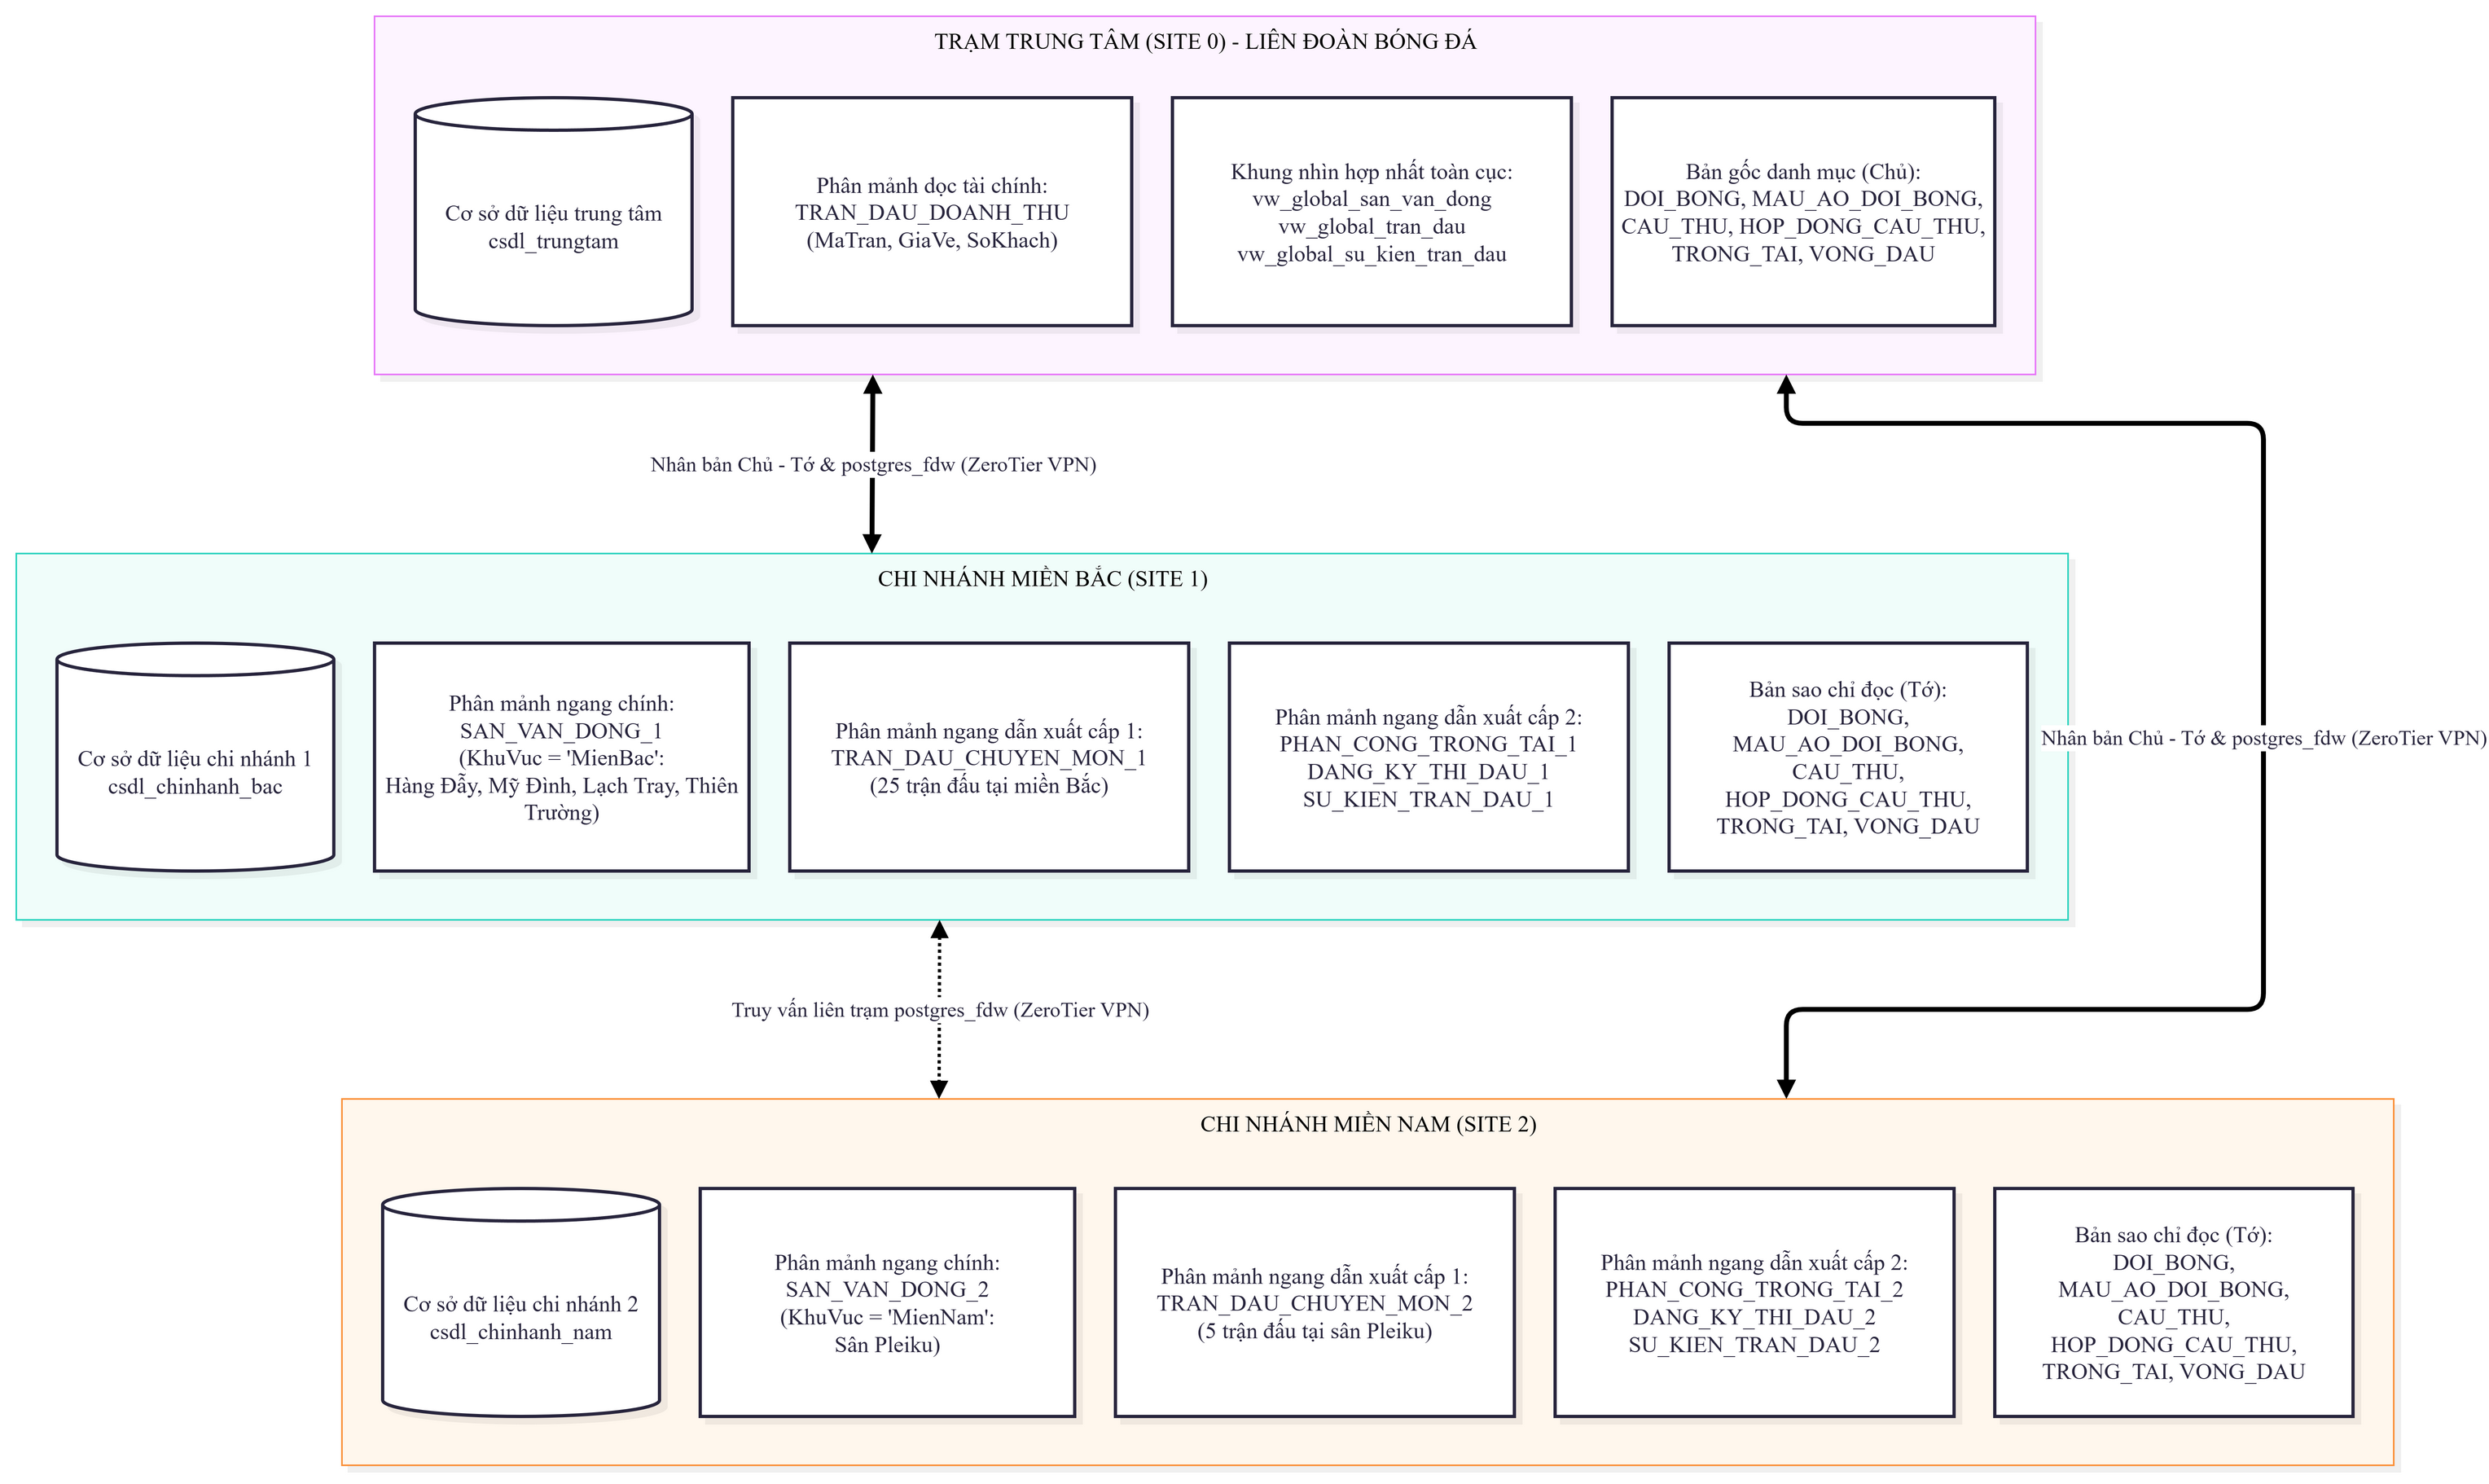
\includegraphics[angle=90, width=0.6\textheight, keepaspectratio]{Figures/DDB.png}
    \caption{Sơ đồ kiến trúc tổng quát của hệ cơ sở dữ liệu phân tán}
    \label{fig:csdl_phan_tan}
\end{figure}

\section{Triển khai kết nối liên trạm và thực nghiệm truy vấn phân tán trên PostgreSQL}

\subsection{Triển khai kết nối liên máy chủ qua mạng riêng ảo ZeroTier và tiện ích mở rộng postgres\_fdw}
Khi triển khai trên ba máy tính vật lý độc lập, các máy chủ được kết nối vào cùng một mạng riêng ảo lớp hai ZeroTier (dải địa chỉ \texttt{10.147.17.0/24}): Trạm Trung tâm (\texttt{10.147.17.10}), Chi nhánh Miền Bắc (\texttt{10.147.17.11}) và Chi nhánh Miền Nam (\texttt{10.147.17.12}). Tại máy chủ Trạm Trung tâm, tiện ích mở rộng \texttt{postgres\_fdw} được kích hoạt để ánh xạ các mảnh dữ liệu từ hai máy chủ miền về hai không gian tên \texttt{site1\_mienbac} và \texttt{site2\_miennam}:

\begin{lstlisting}[language=SQL, caption={Cấu hình kết nối liên máy chủ qua mạng ảo ZeroTier bằng postgres\_fdw}]
CREATE EXTENSION IF NOT EXISTS postgres_fdw;

CREATE SERVER srv_site1_mienbac FOREIGN DATA WRAPPER postgres_fdw
    OPTIONS (host '10.147.17.11', port '5432', dbname 'vleague_bac');
CREATE SERVER srv_site2_miennam FOREIGN DATA WRAPPER postgres_fdw
    OPTIONS (host '10.147.17.12', port '5432', dbname 'vleague_nam');

CREATE USER MAPPING FOR postgres SERVER srv_site1_mienbac
    OPTIONS (user 'postgres', password 'secret_pwd');
CREATE USER MAPPING FOR postgres SERVER srv_site2_miennam
    OPTIONS (user 'postgres', password 'secret_pwd');

IMPORT FOREIGN SCHEMA public FROM SERVER srv_site1_mienbac INTO site1_mienbac;
IMPORT FOREIGN SCHEMA public FROM SERVER srv_site2_miennam INTO site2_miennam;
\end{lstlisting}

Bên cạnh cấu hình đa máy chủ vật lý ở trên, kịch bản \texttt{06\_distributed\_simulation.sql} của đề tài đồng thời hỗ trợ khởi tạo trực tiếp ba không gian tên (\texttt{site0\_trungtam}, \texttt{site1\_mienbac}, \texttt{site2\_miennam}) trên cùng một thực thể PostgreSQL để phục vụ kiểm thử tức thì toàn bộ các phép toán đại số phân mảnh.

\subsection{Kịch bản khởi tạo phân mảnh theo đúng biểu thức đại số quan hệ}
Các câu lệnh dưới đây thực thi chính xác phân mảnh dọc bảng \texttt{TRAN\_DAU}, phân mảnh ngang nguyên thủy bảng \texttt{SAN\_VAN\_DONG} theo vị từ \texttt{KhuVuc}, và chuỗi phân mảnh ngang dẫn xuất hai cấp bằng phép bán kết nối (\texttt{WHERE EXISTS}):

\begin{lstlisting}[language=SQL, caption={Khởi tạo các phân mảnh dọc, phân mảnh ngang nguyên thủy và phân mảnh dẫn xuất}]
-- 1. Phan manh doc: TRAN_DAU_DOANH_THU luu tru doc quyen tai Site 0
CREATE TABLE site0_trungtam.TRAN_DAU_DOANH_THU (
    MaTran VARCHAR(10) PRIMARY KEY,
    GiaVe DECIMAL(12, 2) NOT NULL CHECK (GiaVe >= 0),
    SoKhach INT NOT NULL DEFAULT 0 CHECK (SoKhach >= 0)
);
INSERT INTO site0_trungtam.TRAN_DAU_DOANH_THU
SELECT MaTran, GiaVe, SoKhach FROM public.TRAN_DAU;

-- 2. Phan manh ngang nguyen thuy: SAN_VAN_DONG theo thuoc tinh KhuVuc
CREATE TABLE site1_mienbac.SAN_VAN_DONG_1 (LIKE public.SAN_VAN_DONG INCLUDING ALL);
INSERT INTO site1_mienbac.SAN_VAN_DONG_1
SELECT * FROM public.SAN_VAN_DONG WHERE KhuVuc = 'MienBac';

CREATE TABLE site2_miennam.SAN_VAN_DONG_2 (LIKE public.SAN_VAN_DONG INCLUDING ALL);
INSERT INTO site2_miennam.SAN_VAN_DONG_2
SELECT * FROM public.SAN_VAN_DONG WHERE KhuVuc = 'MienNam';

-- 3. Phan manh ngang dan xuat cap 1: TRAN_DAU_CHUYEN_MON ban ket noi voi SAN_VAN_DONG
CREATE TABLE site1_mienbac.TRAN_DAU_CHUYEN_MON_1 AS
SELECT t.MaTran, t.MaVong, t.MaDoiNha, t.MaDoiKhach, t.MaSan, t.NgayGio,
       t.BanThangNha, t.BanThangKhach, t.TheVangNha, t.TheVangKhach, t.TheDoNha, t.TheDoKhach, t.TrangThai
FROM public.TRAN_DAU t
WHERE EXISTS (SELECT 1 FROM site1_mienbac.SAN_VAN_DONG_1 s WHERE s.MaSan = t.MaSan);

CREATE TABLE site2_miennam.TRAN_DAU_CHUYEN_MON_2 AS
SELECT t.MaTran, t.MaVong, t.MaDoiNha, t.MaDoiKhach, t.MaSan, t.NgayGio,
       t.BanThangNha, t.BanThangKhach, t.TheVangNha, t.TheVangKhach, t.TheDoNha, t.TheDoKhach, t.TrangThai
FROM public.TRAN_DAU t
WHERE EXISTS (SELECT 1 FROM site2_miennam.SAN_VAN_DONG_2 s WHERE s.MaSan = t.MaSan);

-- 4. Phan manh ngang dan xuat cap 2: PHAN_CONG_TRONG_TAI, DANG_KY_THI_DAU va SU_KIEN_TRAN_DAU
-- (A) Tai Site 1 (Mien Bac): 25 tran mien Bac
CREATE TABLE site1_mienbac.PHAN_CONG_TRONG_TAI_1 (LIKE public.PHAN_CONG_TRONG_TAI INCLUDING ALL);
INSERT INTO site1_mienbac.PHAN_CONG_TRONG_TAI_1
SELECT pc.* FROM public.PHAN_CONG_TRONG_TAI pc
WHERE EXISTS (SELECT 1 FROM site1_mienbac.TRAN_DAU_CHUYEN_MON_1 t WHERE t.MaTran = pc.MaTran);

CREATE TABLE site1_mienbac.DANG_KY_THI_DAU_1 (LIKE public.DANG_KY_THI_DAU INCLUDING ALL);
INSERT INTO site1_mienbac.DANG_KY_THI_DAU_1
SELECT dk.* FROM public.DANG_KY_THI_DAU dk
WHERE EXISTS (SELECT 1 FROM site1_mienbac.TRAN_DAU_CHUYEN_MON_1 t WHERE t.MaTran = dk.MaTran);

CREATE TABLE site1_mienbac.SU_KIEN_TRAN_DAU_1 (LIKE public.SU_KIEN_TRAN_DAU INCLUDING ALL);
INSERT INTO site1_mienbac.SU_KIEN_TRAN_DAU_1
SELECT sk.* FROM public.SU_KIEN_TRAN_DAU sk
WHERE EXISTS (SELECT 1 FROM site1_mienbac.TRAN_DAU_CHUYEN_MON_1 t WHERE t.MaTran = sk.MaTran);

-- (B) Tai Site 2 (Mien Nam): 5 tran mien Nam
CREATE TABLE site2_miennam.PHAN_CONG_TRONG_TAI_2 (LIKE public.PHAN_CONG_TRONG_TAI INCLUDING ALL);
INSERT INTO site2_miennam.PHAN_CONG_TRONG_TAI_2
SELECT pc.* FROM public.PHAN_CONG_TRONG_TAI pc
WHERE EXISTS (SELECT 1 FROM site2_miennam.TRAN_DAU_CHUYEN_MON_2 t WHERE t.MaTran = pc.MaTran);

CREATE TABLE site2_miennam.DANG_KY_THI_DAU_2 (LIKE public.DANG_KY_THI_DAU INCLUDING ALL);
INSERT INTO site2_miennam.DANG_KY_THI_DAU_2
SELECT dk.* FROM public.DANG_KY_THI_DAU dk
WHERE EXISTS (SELECT 1 FROM site2_miennam.TRAN_DAU_CHUYEN_MON_2 t WHERE t.MaTran = dk.MaTran);

CREATE TABLE site2_miennam.SU_KIEN_TRAN_DAU_2 (LIKE public.SU_KIEN_TRAN_DAU INCLUDING ALL);
INSERT INTO site2_miennam.SU_KIEN_TRAN_DAU_2
SELECT sk.* FROM public.SU_KIEN_TRAN_DAU sk
WHERE EXISTS (SELECT 1 FROM site2_miennam.TRAN_DAU_CHUYEN_MON_2 t WHERE t.MaTran = sk.MaTran);
\end{lstlisting}

\subsection{Tái thiết toàn cục và tối ưu hóa truy vấn phân tán tại Trạm Trung tâm}
Tại Trạm Trung tâm, các khung nhìn toàn cục tái thiết lại quan hệ gốc bằng phép hợp (\texttt{UNION ALL}) kết hợp phép nối dọc trên khóa chính \texttt{MaTran}. Đặc biệt, đối với truy vấn thống kê Vua phá lưới toàn giải trên kiến trúc phân tán, thay vì kéo toàn bộ các bản ghi sự kiện từ hai trạm miền về Trung tâm rồi mới thực hiện phép gom nhóm, câu truy vấn được tối ưu bằng kỹ thuật \textbf{đẩy phép gom nhóm cục bộ xuống từng trạm miền}, sau đó Trạm Trung tâm chỉ cộng tổng kết quả thu gọn từ hai miền và kết nối với danh mục cầu thủ:

\begin{lstlisting}[language=SQL, caption={Tái thiết toàn cục và tối ưu hóa truy vấn Vua phá lưới phân tán}]
-- Khung nhin tai thiet toan cuc TRAN_DAU (Hop ngang + Noi doc tren MaTran)
CREATE OR REPLACE VIEW site0_trungtam.vw_global_tran_dau AS
SELECT 
    cm.MaTran, cm.MaVong, cm.MaDoiNha, cm.MaDoiKhach, cm.MaSan, cm.NgayGio,
    dt.GiaVe, dt.SoKhach,
    cm.BanThangNha, cm.BanThangKhach, cm.TheVangNha, cm.TheVangKhach, 
    cm.TheDoNha, cm.TheDoKhach, cm.TrangThai
FROM (
    SELECT * FROM site1_mienbac.TRAN_DAU_CHUYEN_MON_1
    UNION ALL
    SELECT * FROM site2_miennam.TRAN_DAU_CHUYEN_MON_2
) cm
JOIN site0_trungtam.TRAN_DAU_DOANH_THU dt ON cm.MaTran = dt.MaTran;

-- Truy van Vua pha luoi phan tan (Day phep gom nhom xuong tung Tram)
WITH BanThangPhanTan AS (
    SELECT local_agg.MaCauThu, SUM(local_agg.SoBan) AS TongBanThang
    FROM (
        SELECT sk1.MaCauThu, COUNT(*) AS SoBan
        FROM site1_mienbac.SU_KIEN_TRAN_DAU_1 sk1
        WHERE sk1.LoaiSuKien = 'BanThang' GROUP BY sk1.MaCauThu
        UNION ALL
        SELECT sk2.MaCauThu, COUNT(*) AS SoBan
        FROM site2_miennam.SU_KIEN_TRAN_DAU_2 sk2
        WHERE sk2.LoaiSuKien = 'BanThang' GROUP BY sk2.MaCauThu
    ) local_agg GROUP BY local_agg.MaCauThu
),
DoiBongHienTai AS (
    SELECT DISTINCT ON (hd.MaCauThu) hd.MaCauThu, db.TenDoi
    FROM site0_trungtam.HOP_DONG_CAU_THU hd
    JOIN site0_trungtam.DOI_BONG db ON hd.MaDoiHienTai = db.MaDoi
    WHERE hd.TrangThai IN ('ChinhThuc', 'ChoMuon')
    ORDER BY hd.MaCauThu, hd.NgayBatDau DESC
)
SELECT ROW_NUMBER() OVER (ORDER BY b.TongBanThang DESC, ct.HoTen ASC) AS XepHang,
       ct.MaCauThu, ct.HoTen, COALESCE(d.TenDoi, 'Tu do') AS TenDoiHienTai, b.TongBanThang
FROM BanThangPhanTan b
JOIN site0_trungtam.CAU_THU ct ON b.MaCauThu = ct.MaCauThu
LEFT JOIN DoiBongHienTai d ON b.MaCauThu = d.MaCauThu
ORDER BY b.TongBanThang DESC, ct.HoTen ASC LIMIT 10;
\end{lstlisting}

Kết quả thực nghiệm xác nhận Chi nhánh Miền Bắc quản lý 4 sân vận động và 25 trận đấu, Chi nhánh Miền Nam quản lý 1 sân vận động và 5 trận đấu, và khung nhìn toàn cục tại Trạm Trung tâm tái thiết chính xác 30 trận đấu cùng đầy đủ thông tin doanh thu bán vé và bảng xếp hạng Vua phá lưới trùng khớp $100\%$ với cơ sở dữ liệu tập trung. Mô hình bảo đảm trọn vẹn tính trong suốt phân mảnh, tính trong suốt vị trí và tính trong suốt nhân bản đối với các ứng dụng khai thác.
